\documentclass[landscape, a0paper, debug]{baposter}

\usepackage{graphicx}
\usepackage{epstopdf}
\usepackage{multirow}
\usepackage{tikz}
\usepackage{url}

\usepackage{amsmath}
\usepackage{amssymb}
\usepackage{relsize}


\begin{document}

\definecolor{silver}{cmyk}{0,0,0,0.3}
\definecolor{yellow}{cmyk}{0,0,0.9,0.0}
\definecolor{reddishyellow}{cmyk}{0,0.22,1.0,0.0}
\definecolor{black}{cmyk}{0,0,0.0,1.0}
\definecolor{darkYellow}{cmyk}{0,0,1.0,0.5}
\definecolor{darkSilver}{cmyk}{0,0,0,0.1}

\definecolor{lightyellow}{cmyk}{0,0,0.3,0.0}
\definecolor{lighteryellow}{cmyk}{0,0,0.1,0.0}
\definecolor{lighteryellow}{cmyk}{0,0,0.1,0.0}
\definecolor{lightestyellow}{cmyk}{0,0,0.05,0.0}

\definecolor{lightblue}{HTML}{9DC2F6}
\definecolor{lightestblue}{HTML}{F3F8FE}
\definecolor{lighterblue}{HTML}{2B7FF2}
\definecolor{darkblue}{HTML}{1D4B8B}
\definecolor{darkerblue}{HTML}{0D75B5}
\definecolor{creamblue}{HTML}{E4EEFB}

\begin{poster}{
    grid=false,
    colspacing=2em,
    columns=3,
    background=none,
    % color style
    bgColorOne=lightblue,
    bgColorTwo=white,
    headerColorOne=darkerblue,
    headerFontColor=white,
    boxColorOne=creamblue,
    boxColorTwo=creamblue,
    borderColor=white,
    % format of textbox
    textborder=roundedleft,
    % format of the header
    eyecatcher=true,
    headerborder=open,
    headerheight=0.08\textheight,
    headershape=roundedright,
    headershade=plain,
    headerfont=\Large\bf\textsf,
    boxshade=plain,
    textfont={\setlength{\parindent}{1.5em}},
    linewidth=2.5pt,
  }
  % eyecatcher section
  {\includegraphics[height=5em]{qrcode}} 
  {
    {\fontsize{30}{30}\bf\textsc{Applying Homomorphic Encryption In The Cloud}}
    \vspace{0.3em}
  }
  {
    \sf Jes\'{u}s Antonio Soto Vel\'{a}zquez\hspace{3em}
    jesus.antoniosv@gmail.com\hspace{3em}
    Universidad Aut\'{o}noma de Nuevo Le\'{o}n, M\'{e}xico
  }
  {{
      \begin{minipage}{20em}
        \hfill
        
\includegraphics[height=4em]{fime}
        \hspace{25pt}
        \includegraphics[height=4em]{logo_uni_lossless}
    \end{minipage}}
  }

  \headerbox{Contribution}{name=contribution,column=0,row=0}{
    This work proposes the \emph{design} and \emph{implementation} of a client-server architecture based software that uses \emph{HElib} to enable homomorphic encryption and perform computations on encrypted data. \\
    The software is used to address the situation in the \emph{case study}.
  }

  \headerbox{Objectives}{name=objectives,column=0,below=contribution}{
    \begin{itemize}
      \renewcommand{\labelitemi}{$>$}
    \item \textbf{Establish} a client-server architecture where homomorphic encryption can be applied.
   \item \textbf{Identify} which factors pose a challenge to apply homomorphic encryption in the cloud.
    \item \textbf{Collect} performance data on the use of homomorphic encryption.
    \end{itemize}
  }

  \headerbox{Case Study}{name=casestudy,column=0,below=objectives}{
    \begin{center}
      \fcolorbox{black}{white}{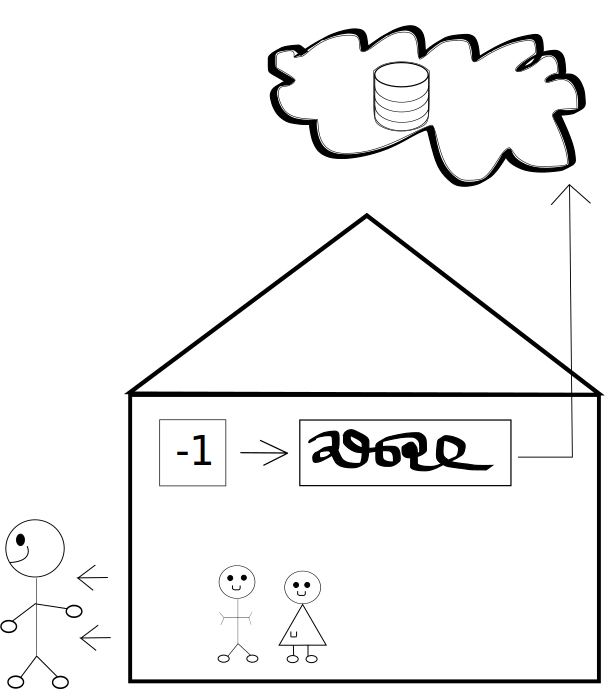
\includegraphics[width=0.60\linewidth]{casestudy}}
    \end{center}
    \vspace{1em}
    Consider a scenario where a household has an expected pattern of activity, so that the resident seeks to ascertain the number of people inside at any time. \\ \\
    As the resident chooses to \textbf{store the value of the counter in the cloud}, he quickly realizes he does not want others to learn of this value, not even the cloud service itself, as to prevent  potential burglars to break in when the household is empty. \\ \\
    Therefore, a mechanism to ensure that the household activity data is available as well as protected needs to be put in place.
  }

  \headerbox{Methodology}{name=methodology,column=1, row=0}{
A client-server architecture was designed and implemented in C++ to address a solution for the presented case study. Homomorphic encryption is enabled by using HElib \cite{brakerski:helib}. Relevant tasks were divided between \textbf{client} and \textbf{server}.
\begin{center}
  \fcolorbox{black}{white}{\includegraphics[width=0.65\linewidth]{architecture}}
\end{center}
\vspace{0.5em}
  }

  \headerbox{Operation Flow}{name=flow,column=1, below=methodology }{
    \begin{center}
      \fcolorbox{black}{white}{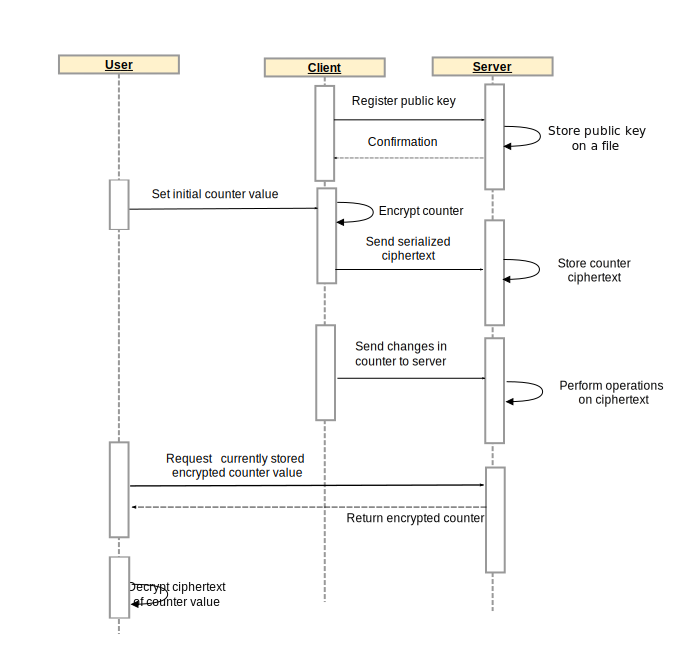
\includegraphics[width=0.95\linewidth]{counter}}
    \end{center}
    \vspace{0.4em}

  }
  
  \headerbox{Experimentation \& Results}{name=results,column=2,row=0}{
    The performance of the system was evaluated by running 20 iterations with distinct values of a security parameter \emph{k} needed for the homomorphic encryption scheme. \\
      The system was evaluated in terms of ciphertext and key size, as well as the time needed for key generation and processing (addition, decryption, encryption).
      \begin{center}
        \fcolorbox{black}{white}{\includegraphics[width=0.95\linewidth]{proc}}
      \end{center}

  }

  \headerbox{Future Work}{name=future,column=2,below=results}{
    \begin{itemize}
    \item Perform more experimentation on the size of the ciphertext.
    \item Secure the communication channel between client and server.
    \item Design a database scheme to store public key-ciphertext pairs.
    \end{itemize}         
  }

  \headerbox{References}{name=ref,column=2,below=future}{
    \smaller
    \vspace{-0.4em}
    \bibliographystyle{ieee}
    \renewcommand{\section}[2]{\vskip 0.05em}
      \begin{thebibliography}{1}\itemsep=-0.01em
      \setlength{\baselineskip}{0.4em}
    \bibitem{brakerski:helib}
        Z.~Brakerski, C.~Gentry, V.Vaikuntanathan.
        \newblock HElib, 2014.
        \newblock \url{https://github.com/shaih/HElib}
      \end{thebibliography}    
  }


  \headerbox{Acknowledgements}{name=ack,column=2,below=ref}{    
    Special thanks to Prof.\ Elisa Schaeffer for providing the graphs of the results and Prof.\ Sara Garza for her support as primary advisor.
  }

  \headerbox{Source Code}{name=code,column=2, below=ack}{
    The code is publicly available at the following repository: \\
    \url{https://github.com/antoniosv/homomorphic-counter}
  }
  
\end{poster}

\end{document}
